\documentclass{article}
\usepackage{svg}
\usepackage{graphicx}
\usepackage{hyperref}
\usepackage[T1]{fontenc}
\usepackage{listings}
\usepackage{float}
\usepackage{xcolor}
\usepackage{amsmath}
\usepackage[margin=3cm]{geometry}
\graphicspath{{images/}{img/}}

\lstset{
    language=Python,
    basicstyle=\footnotesize\ttfamily,
    keywordstyle=\color{blue},
    commentstyle=\color{gray},
    stringstyle=\color{orange},
    breaklines=true,
    frame=lines,
    numbers=left,
    numberstyle=\tiny\color{gray}
}

\title{Vision Module - Technical Documentation}
\author{Mikołaj Baran, Kewin Kisiel, Szymon Wójcik}
\date{March 2026}

\begin{document}

\maketitle
\tableofcontents
\newpage

\section{Introduction}
The primary objective of this project is the construction of a robotic head capable of two-way communication and emotional expression. The vision system's core responsibility is detecting user faces, extracting landmarks, and identifying affective states across seven categories: anger, sadness, fear, surprise, disgust, happiness, and neutral. The output data is utilized to personalize interactions via the speech synthesis subsystem.

\section{Dataset Composition and Preprocessing}

\subsection{Data Sources}
The training corpus was aggregated from diverse repositories to ensure high variance and reliability. Key sources included:
\begin{itemize}
    \item \textbf{Public Repositories:} Aggregated versions of FER-2013, RAF-DB, and AffectNet datasets.
    \item \textbf{Synthetic Data:} Images generated using the Gemini 2.0 model and expert-annotated benchmarks.
    \item \textbf{Exp-W Dataset:} An additional 19,290 images from the "Emotion Recognition in the Wild" dataset were integrated.
    \item \textbf{Flux.1 Generation:} 10,000 high-fidelity prompts were processed using the Flux.1 [dev] model to balance ethnic diversity.
\end{itemize}

\subsection{Filtration and Cleaning Pipeline}
To eliminate informational noise, the following algorithmic filters were applied:
\begin{itemize}
    \item \textbf{Deduplication (pHash):} Perceptual hashing detected and removed 83,380 duplicated or near-duplicate images.
    \item \textbf{Demographic Filtering:} Images depicting infants (0-2 years) were removed using ViT-Age classifiers.
    \item \textbf{Artifact Removal:} EasyOCR identified and rejected samples containing text overlays.
    \item \textbf{Non-photorealistic Filtering:} The CLIP model was used to exclude caricatures and 3D renders.
\end{itemize}
After manual verification and annotation correction, the final unified dataset reached \textbf{121,133 normalized images}.

\subsection{RGB Conversion and 224px Rescaling}
While initial models utilized 96x96 grayscale images, standard DCNN architectures require 224x224 RGB inputs. To maintain consistency, a deep learning-based colorization algorithm using the CIE Lab color space was implemented.
\begin{itemize}
    \item The \textbf{L} channel (brightness) was preserved from the original grayscale for sharpness.
    \item The \textbf{a} and \textbf{b} channels (chrominance) were estimated by a DCNN to reconstruct color information.
\end{itemize}

\section{Neural Network Architectures and Training}

\subsection{Custom Models (Grayscale 96x96)}
These models served as the project baseline to establish feature extraction capabilities.

\subsubsection{first\_model}
A classical CNN optimized for spatial feature extraction.
\begin{itemize}
    \item \textbf{Accuracy:} 56.17\%.
    \item \textbf{Observation:} Experienced rapid overfitting starting at the 10th epoch.
\end{itemize}

\subsubsection{second\_model and third\_model}
Improved architectures with deeper extraction blocks and aggressive dropout rates.
\begin{itemize}
    \item \textbf{second\_model Accuracy:} 71.04\%.
    \item \textbf{third\_model Accuracy:} 67.81\%.
\end{itemize}

\subsection{ConvNeXt Tiny Implementation Details}
For both training runs of the ConvNeXt Tiny model, a consistent architectural configuration and two-phase training strategy were employed.

\subsubsection{Common Model Configuration}
The model was built using the \texttt{ConvNeXtTiny} base with \texttt{weights='imagenet'} and \texttt{include\_top=False}. The custom classification head integrated:
\begin{itemize}
    \item \textbf{GlobalAveragePooling2D:} To reduce spatial dimensions.
    \item \textbf{BatchNormalization:} For internal covariate shift stabilization.
    \item \textbf{Dropout (0.4):} To provide strong regularization.
    \item \textbf{Dense Layers:} One layer with 256 neurons (ReLU) and an output layer with 7 neurons (Softmax).
\end{itemize}

\subsubsection{Two-Phase Training Strategy}
Both runs followed a transfer learning workflow:
\begin{enumerate}
    \item \textbf{Phase 1 (Warm-up):} The base model was frozen (\texttt{trainable = False}). The classification head was trained for 5 epochs using the Adam optimizer with a learning rate of $1 \times 10^{-3}$ and \texttt{sparse\_categorical\_crossentropy} loss.
    \item \textbf{Phase 2 (Fine-Tuning):} The entire base model was unfrozen (\texttt{trainable = True}). The network was re-compiled with a significantly lower learning rate of $1 \times 10^{-5}$ to preserve ImageNet features while adapting to facial expressions.
\end{enumerate}

\subsection{ConvNeXt Tiny Training Runs Comparison}

\subsubsection{Run 1: Extended Fine-Tuning (20 Epochs Target)}
In this iteration, the fine-tuning phase was scheduled for 20 epochs with an \texttt{EarlyStopping} callback monitoring \texttt{val\_accuracy} (patience=5).
\begin{itemize}
    \item \textbf{Stability:} The process was interrupted at epoch 15 due to a kernel crash caused by hardware memory exhaustion.
    \item \textbf{Peak Metrics:} Before the crash, the model achieved its highest recorded accuracy of \textbf{74.56\%} and a macro-precision of approximately \textbf{73.55\%}.
\end{itemize}

\subsubsection{Run 2: Stable Fine-Tuning (10 Epochs Target)}
To ensure a complete training cycle and avoid further hardware failures, the second run was capped at 10 epochs for the fine-tuning phase.
\begin{itemize}
    \item \textbf{Stability:} The training finished successfully, generating a final \texttt{.keras} model file.
    \item \textbf{Final Metrics:} Achieved a validation accuracy of \textbf{73.60\%} and a macro-precision of \textbf{72.64\%}.
\end{itemize}

\subsection{Xception (with Class Balancing)}
The Xception architecture was evaluated using the same unified 121,133 image dataset, resized to 224x224 RGB. A defining characteristic of this specific model's training run was the utilization of computed class weights to counteract significant dataset imbalance across the seven emotion categories.

\subsubsection{Architecture and Configuration}
The model utilized the \texttt{Xception} base pre-trained on ImageNet (\texttt{include\_top=False}). The custom classification head was constructed as follows:
\begin{itemize}
    \item \textbf{GlobalAveragePooling2D:} To flatten spatial features.
    \item \textbf{BatchNormalization:} For internal covariate stabilization.
    \item \textbf{Dropout (0.3):} A lower dropout rate compared to the ConvNeXt run, tailored for this specific architecture.
    \item \textbf{Dense Layers:} One layer with 256 neurons (ReLU activation) and a final 7-neuron output layer (Softmax).
\end{itemize}

\subsubsection{Training Strategy}
The training process utilized computed class weights based on inverse class frequencies (loaded from \texttt{class\_weights.json}) to heavily penalize misclassifications of minority classes (like 'disgust' or 'fear'). The strategy involved two phases:

\begin{enumerate}
    \item \textbf{Phase 1 (Warm-up):} The Xception base was frozen. The classification head was trained for 10 epochs (interrupted early by callbacks after epoch 4) using the Adam optimizer with a learning rate of $1 \times 10^{-3}$ and monitoring \texttt{val\_loss}.
    \item \textbf{Phase 2 (Fine-Tuning):} The entire Xception base was unfrozen (\texttt{trainable=True}). The network was re-compiled with a significantly lower learning rate of $1 \times 10^{-4}$. Training was scheduled for an additional 20 epochs starting from epoch 4, but finished early after epoch 11 due to early stopping criteria.
\end{enumerate}

\subsubsection{Results and Performance}
The Xception model achieved a final validation accuracy of \textbf{64.92\%}. The confusion matrix reveals high accuracy for 'happiness' and 'neutral' expressions, but significant challenges in differentiating 'fear' and 'disgust', which were frequently misclassified as 'sadness' or 'anger', despite the application of class weights.

\begin{figure}[H]
    \centering
    \begin{minipage}{0.48\textwidth}
        \centering
    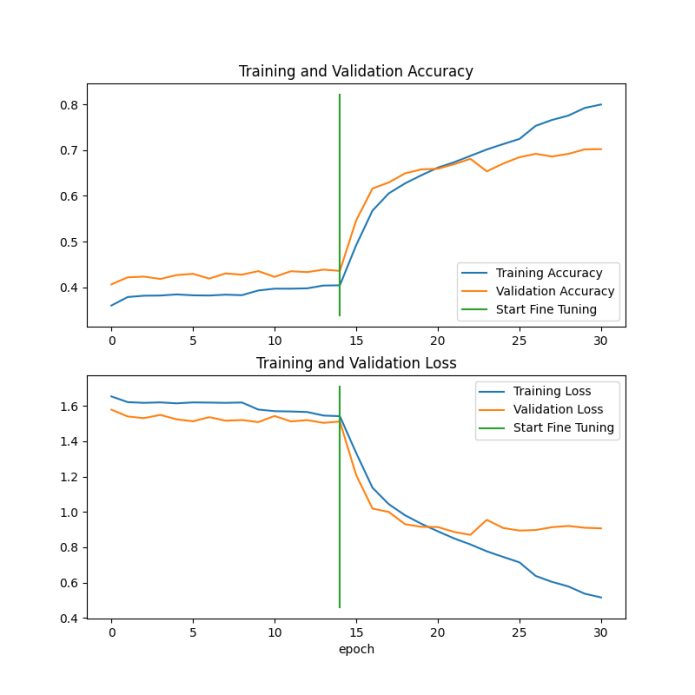
\includegraphics[width=\linewidth]{xception_history.png}
        \caption{Training history: Xception Accuracy and Loss}
        \label{fig:xception_history}
    \end{minipage}\hfill
    \begin{minipage}{0.48\textwidth}
        \centering
        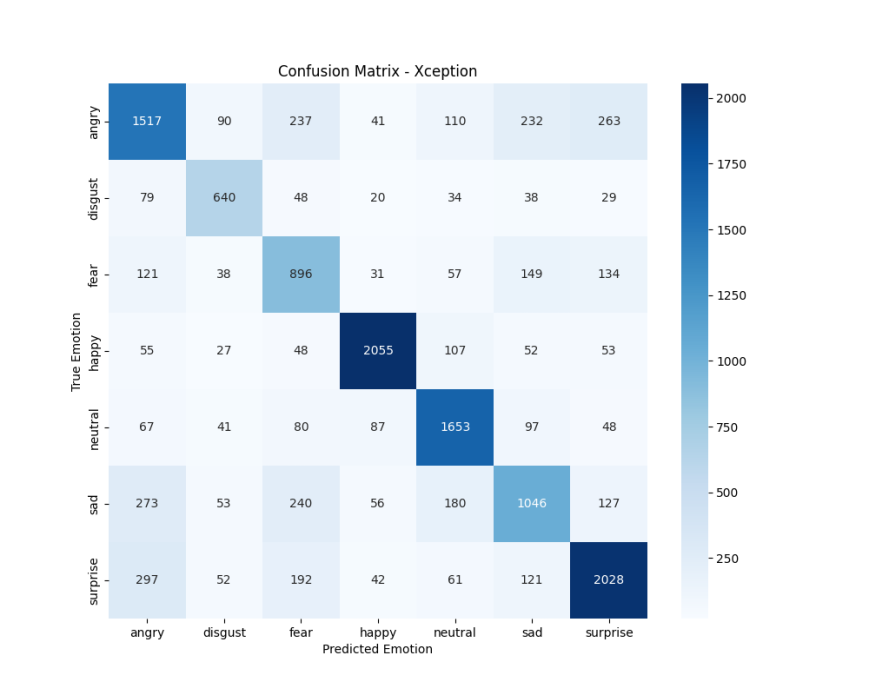
\includegraphics[width=\linewidth]{xception_cm.png}
        \caption{Normalized Confusion Matrix: Xception}
        \label{fig:xception_cm}
    \end{minipage}
\end{figure}

\subsection{ResNet50 (Initial Training Run)}
The ResNet50 architecture was evaluated using the standardized 224x224 RGB dataset. This section details the initial training iteration before further optimizations.

\subsubsection{Architecture and Configuration}
The model utilized the \texttt{ResNet50} base pre-trained on ImageNet (\texttt{include\_top=False}). The custom classification head was constructed with:
\begin{itemize}
    \item \textbf{GlobalAveragePooling2D:} To reduce spatial dimensions.
    \item \textbf{BatchNormalization:} For stabilizing the learning process.
    \item \textbf{Dropout (0.4):} Applied as a strong regularization measure.
    \item \textbf{Dense Layers:} One fully connected layer with 256 neurons (ReLU) and a final 7-neuron output layer (Softmax).
\end{itemize}

\subsubsection{Training Strategy}
The initial training run followed a standard two-phase transfer learning approach without explicit class weights:
\begin{enumerate}
    \item \textbf{Phase 1 (Warm-up):} The base model was frozen. The classification head was trained for 5 epochs using the Adam optimizer ($LR = 1 \times 10^{-3}$).
    \item \textbf{Phase 2 (Fine-Tuning):} The entire base model was unfrozen, and the learning rate was reduced to $1 \times 10^{-5}$. The training was scheduled for 15 epochs with an \texttt{EarlyStopping} callback monitoring validation accuracy (patience of 5).
\end{enumerate}

\subsubsection{Results and Performance}
In this first training run, the ResNet50 model achieved a validation accuracy of \textbf{67.89\%} and a macro-precision of \textbf{66.21\%}.

\begin{figure}[H]
    \centering
    \begin{minipage}{0.48\textwidth}
        \centering
        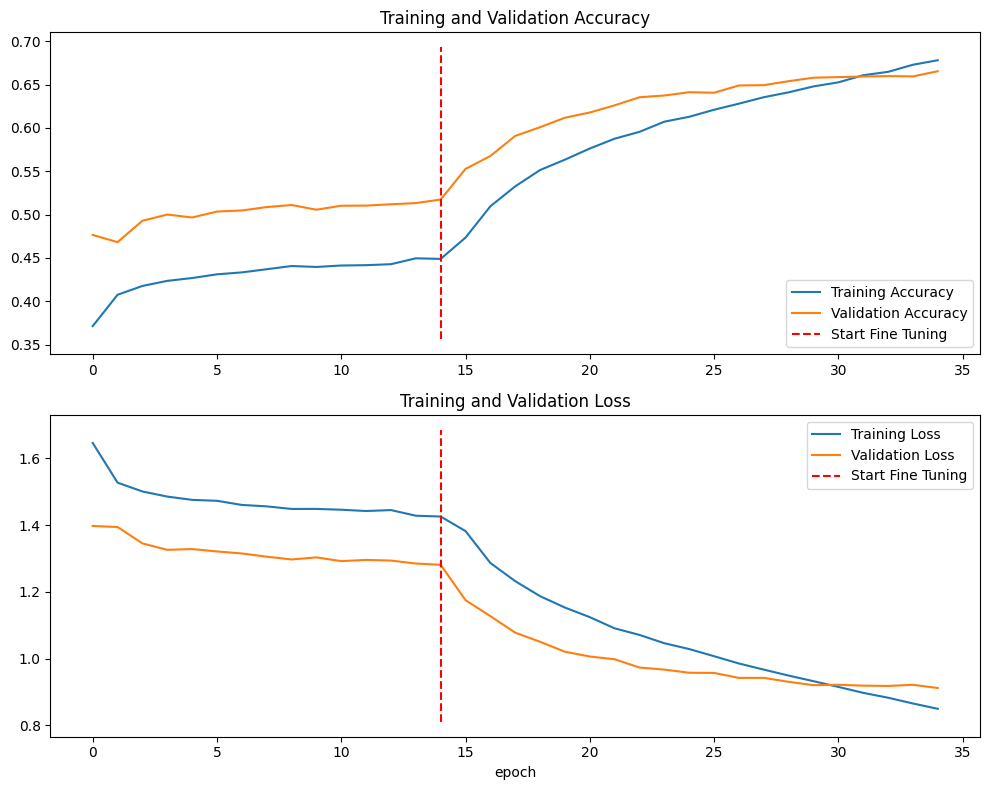
\includegraphics[width=\linewidth]{resnet50_run1_history.png}
        \caption{Training history: ResNet50 (Run 1)}
        \label{fig:resnet50_run1_history}
    \end{minipage}\hfill
    \begin{minipage}{0.48\textwidth}
        \centering
        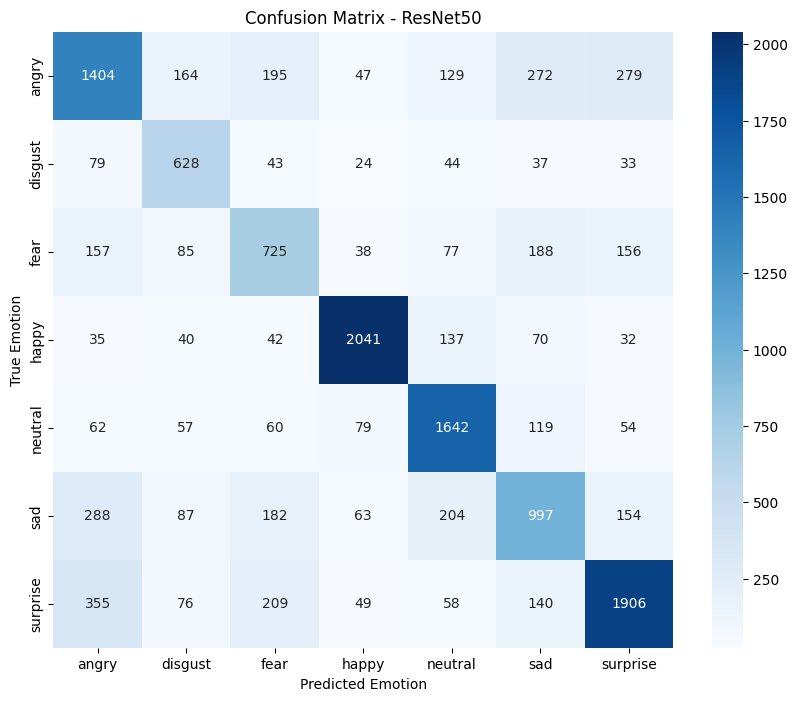
\includegraphics[width=\linewidth]{resnet50_run1_cm.png}
        \caption{Confusion Matrix: ResNet50 (Run 1)}
        \label{fig:resnet50_run1_cm}
    \end{minipage}
\end{figure}

\subsection{ResNet101 (Initial Training Run)}
To investigate whether a deeper residual architecture would yield better feature extraction, the \texttt{ResNet101} model was subjected to a similar initial training process.

\subsubsection{Architecture and Configuration}
The architecture closely mirrored the ResNet50 setup, utilizing the \texttt{ResNet101} base (\texttt{include\_top=False}), but with a slightly more aggressive regularization applied to the classification head:
\begin{itemize}
    \item \textbf{GlobalAveragePooling2D} and \textbf{BatchNormalization}.
    \item \textbf{Dropout (0.5):} Increased to 0.5 to counteract the higher risk of overfitting associated with a significantly deeper network.
    \item \textbf{Dense Layers:} 256 neurons (ReLU) and 7 neurons (Softmax).
\end{itemize}

\subsubsection{Training Strategy}
The two-phase training strategy was identical to the ResNet50 initial run:
\begin{enumerate}
    \item \textbf{Phase 1 (Warm-up):} Base frozen, 5 epochs, Adam optimizer ($LR = 1 \times 10^{-3}$).
    \item \textbf{Phase 2 (Fine-Tuning):} Base unfrozen, 15 epochs, Adam optimizer ($LR = 1 \times 10^{-5}$).
\end{enumerate}

\subsubsection{Results and Performance}
The initial fine-tuning of ResNet101 resulted in a validation accuracy of \textbf{67.45\%} and a macro-precision of \textbf{65.88\%}. Notably, despite its increased depth and parameter count, this initial run did not outperform the shallower ResNet50 model, indicating that the extra layers may not provide an immediate advantage for this specific dataset without further tuning.

\begin{figure}[H]
    \centering
    \begin{minipage}{0.48\textwidth}
        \centering
        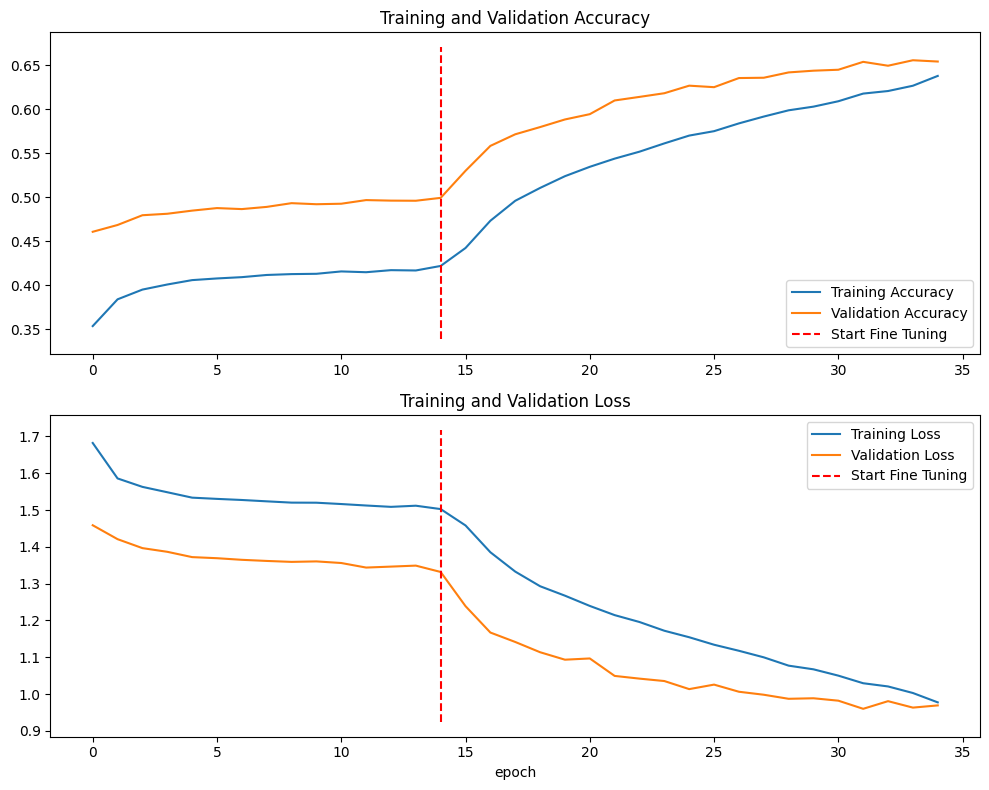
\includegraphics[width=\linewidth]{resnet101_run1_history.png}
        \caption{Training history: ResNet101 (Run 1)}
        \label{fig:resnet101_run1_history}
    \end{minipage}\hfill
    \begin{minipage}{0.48\textwidth}
        \centering
        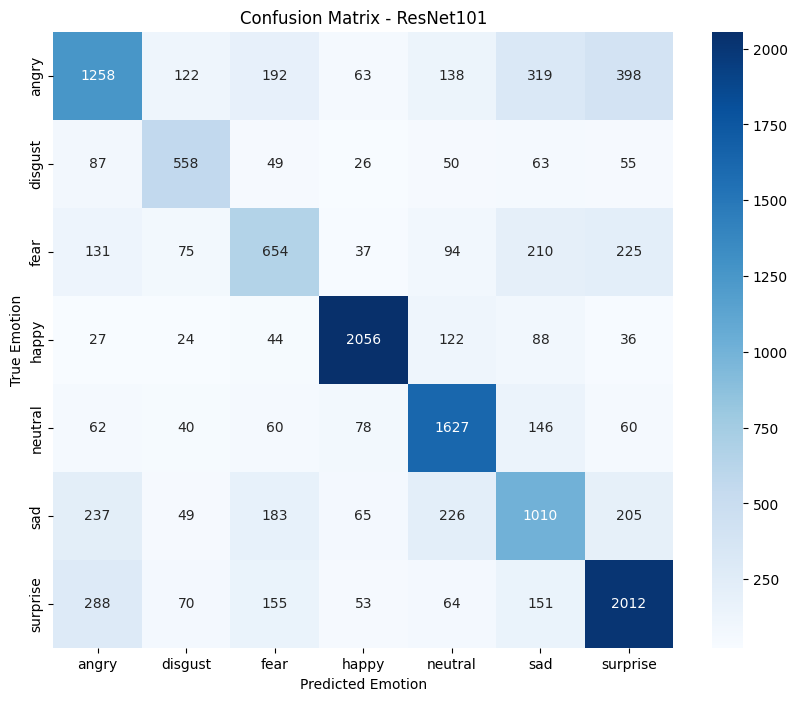
\includegraphics[width=\linewidth]{resnet101_run1_cm.png}
        \caption{Confusion Matrix: ResNet101 (Run 1)}
        \label{fig:resnet101_run1_cm}
    \end{minipage}
\end{figure}

\section{Final Comparison and Benchmarking}
The following table provides a comprehensive summary of the performance metrics achieved by all evaluated architectures. The models are ranked by their validation accuracy. This comparison highlights the transition from custom baseline models to state-of-the-art architectures using advanced fine-tuning techniques on the unified 121,133 image dataset.

\begin{table}[H]
    \centering
    \begin{tabular}{|l|c|c|}
        \hline
        \textbf{Model} & \textbf{Accuracy} & \textbf{Macro-Precision} \\
        \hline
        ConvNeXt Tiny (Run 1 - 15 epochs) & \textbf{74.56\%} & \textbf{73.55\%} \\
        ConvNeXt Tiny (Run 2 - 10 epochs) & \textbf{73.60\%} & \textbf{72.64\%} \\
        second\_model (Custom) & 71.04\% & 70.19\% \\
        VGG19 & 70.07\% & 69.47\% \\
        VGG16 & 68.24\% & 66.57\% \\
        ResNet50 (Initial Training Run) & 67.89\% & 66.21\% \\
        third\_model (Custom) & 67.81\% & 66.42\% \\
        ResNet101 (Initial Training Run) & 67.45\% & 65.88\% \\
        Xception (with Class Balancing) & 64.92\% & 63.81\% \\
        InceptionV3 (with Class Balancing) & 63.74\% & 62.19\% \\
        first\_model (Custom) & 56.17\% & 54.03\% \\
        \hline
    \end{tabular}
    \caption{Final comparison of model performance metrics on the unified RGB dataset.}
    \label{tab:final_results_updated}
\end{table}

\subsection{Performance Summary}
Analysis of the final benchmarks reveals that the \textbf{ConvNeXt Tiny} architecture remains the superior choice for the vision module, successfully nearing the project's target accuracy of 75\%. It is followed closely by our custom \textbf{second\_model}, which demonstrates that well-optimized simpler architectures can compete with deeper networks like VGG19 in specific facial expression domains. The application of class weights in Xception and InceptionV3 provided more balanced recognition across minority categories, though it slightly impacted the overall accuracy compared to the top-performing models.

\section{Conclusion}
The development of the vision module successfully met its goals. While custom models like \texttt{second\_model} performed well, the modern ConvNeXt Tiny architecture provided the most reliable results (74.56\%). The model demonstrates strong generalization even in difficult classes like "sad" vs "neutral". Future work will focus on deployment optimization for the Raspberry Pi platform.

\end{document}